\documentclass[../dissertation.tex]{subfiles}

\begin{document}

\subsection{Experiment 2 - Rebooting}

\paragraph{Introduction} It was seen while running Experiment 1 that at higher frequencies running the same experiment multiple times in a row would give erratic results. The first run might have reasonable performance, then repeating it would give poorer results, and the third run would be reasonable again. It was suggested in conversations that the behaviour could be caused by operating system buffers filling up and then not being purged until either full, or being cleared by some other process. Rebooting the systems has the opportunity to affect performance by stopping any background processes, interrupting slow processing messages from previous runs, and resetting any message caches and buffers in memory.

%Experiment 2 was an investigation in to whether the performance of ROS messages was affected by previous messages sent on the system. This was tested by comparing the performance of ROS messages of 5 consecutive message passing runs vs 5 message passing runs with system reboots between runs. This was repeated at 1KHz, 4KHz, 7KHz, and 10Khz frequencies for two reasons. The first was to investigate whether areas in which we observed consistent performance before would exhibit any difference between reboot and no reboot. Secondly, it would give further insight in to where the exact barrier between `good, consistent performance' and `poor, erratic performance' is.

\paragraph{Objective} Experiment 2's primary objective was to evaluate whether the performance of ROS' inter-robot communication was being affected by not fully rebooting the sending machine and the echoer machine in between experimental runs - in other words, whether the performance of ROS messages was affected by previous messages sent on the system. Experiment 2 also had the secondary objective of providing greater insight in to where the exact barrier between `good, consistent performance' and `poor, erratic performance' is - as in Experiment 1 there was a jump in latency between 1KHz and 10KHz message frequencies.

\paragraph{Hypothesis} The result of the experiment was hypothesised to demonstrate no significant difference between rebooting and not-rebooting at any message frequency. It is expected that the erratic performance between runs is more likely to be caused by interference from uncontrolled background processes, or a resource bottleneck such as CPU speed.

\paragraph{Materials and Methodology} The hardware set-up is identical as Experiment 1 (see Section \ref{exp-1}), however the methodology is different. This experiment compares two set-ups: the first, `Full Reboot' involves executed a full system reboot of all involved Raspberry Pis between each experiment run, and the second, `No Reboot' involves simply waiting a few seconds before executing the next run. Both configurations are to be run 5 times in total. The messages being sent are also identical as Experiment 1.

\paragraph{Results and Discussion} Figure \ref{exp2-1khz-mean} demonstrates that for relatively low message frequencies the mean message latency was consistently 1 - 1.5ms (the peak around message 500 in the full reboot data was due to a single erroneous run, possibly indicating a system update or some other scheduled background process took place). Figure \ref{exp2-4khz-mean} is characteristic of the higher frequency runs - the no reboot runs generally gave equal or better performance compared to the full reboot runs. See Appendix \ref{exp2-appendix-results} for other mean graphs, and individual run graphs.

\textit{We can conclude from this that rebooting the host systems between experimental runs would result in worse communication performance for ROS, thus in future experiments the host systems will not be rebooted between runs. Secondly, we can also conclude that the exact frequency that message latencies begin increasing above nominal values is somewhere between 1KHz and 4KHz.}

\begin{figure}[H]
\centering
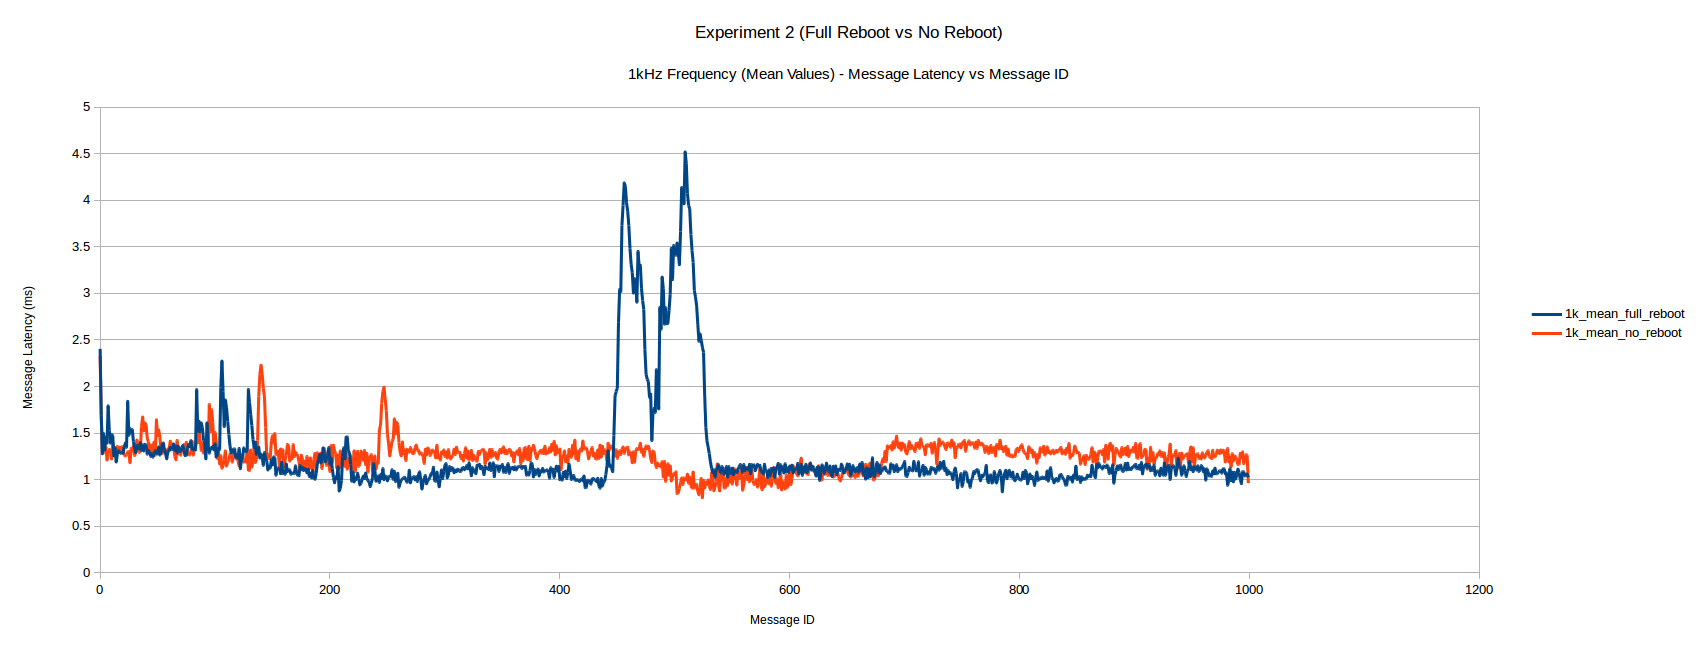
\includegraphics[width=\textwidth]{images/experiment2/1khz-mean.png}
\caption{Experiment 2 - Mean Message Latency 1KHz Message Frequency}
\label{exp2-1khz-mean}
\end{figure}

\begin{figure}[H]
\centering
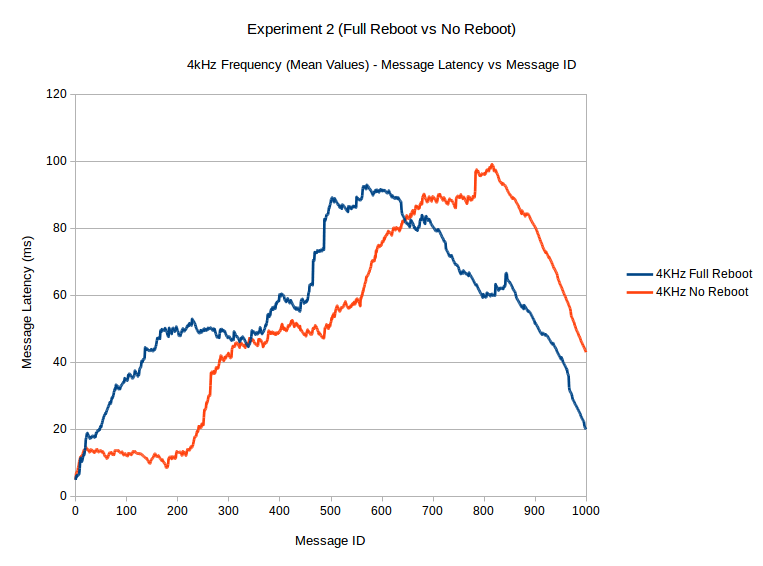
\includegraphics[width=\textwidth]{images/experiment2/4khz-mean.png}
\caption{Experiment 2 - Mean Message Latency 4KHz Message Frequency}
\label{exp2-4khz-mean}
\end{figure}

\end{document}
